%\documentclass[a4paper]{article}
\documentclass[runningheads]{llncs}
\usepackage[margin=1.2in]{geometry}

\usepackage{hyperref}
\usepackage{indentfirst}

\usepackage{enumitem}
\newlist{steps}{enumerate}{1}
\setlist[steps, 1]{label = Step \arabic*:}

\usepackage{graphicx}
\graphicspath{ {./images/} }

\title{Part2Part \& Chord}
\author{Oloieri Alexandru, IIA2}
\institute{Facultatea de Informatică Iași}
\date{2 Decembrie 2019}

\begin{document}

\maketitle

\begin{abstract}

\centering
Acest document prezintă o posibilă structură, precum şi idei de implementare a unei reţele descentralizate de partajare a fişierelor, ce implementează protocolul/algoritmul \textbf{Chord} pentru găsirea rapidă a nodurilor din reţea.

\end{abstract}

\section{Introducere}

Peer-to-peer (P2P) este o arhitectură de reţea în care nodurile sunt relativ egale, în sensul că fiecare nod este, în principiu, capabil să realizeze funcţiile specifice reţelei. În aceste sisteme descentralizate o provocare este găsirea unui nod din reţea în mod eficient, întrucât soluţia evidentă (în care fiecare nod din reţea ştie despre orice alt nod) este ineficientă atât din punct de vedere al memoriei, cât şi al timpului de execuţie. 

O metodă pentru eficientizarea operaţiilor în reţelele P2P este utilizarea tabelelor de dispersie distribuite (tabele hash distribuite - DTH). Pentru acestea au fost inventate mai multe protocoale, în acest document urmând să fie descris protocolul \textbf{Chord} şi modul în care poate fi integrat într-o reţea descentralizată ce are ca scop distribuirea fişierelor între nodurile acesteia.

\section{Tehnologii utilizate}

Aplicaţia va fi implementată în limbajul \textbf{C++}, întrucât posibilitatea de a utiliza elemente ale programării orientate obiect uşurează mult implementarea.

Pentru comunicarea în reţea va fi utilizat protocolul \textbf{TCP/IP}, pentru că viteza şi corectitudinea operaţiilor de căutarea a unor elemente în tabela hash distribuită pot fi afectate în cazul în care mesajele ce ajung la unul dintre servere sunt eronate, nu respectă ordinea în care au fost trimise sau, şi mai rău, sunt pierdute. Pentru programarea în reţea va fi folosit API-ul Socket-BSD (Berkeley System Distribution).

Pentru ca serverele din reţea să fie concurente, acestea vor crea câte un thread pentru fiecare client ce se conectează, iar pentru asta va fi utilizată librăria \textbf{pthread} din limbajul \textbf{C}.

Vor fi utilizate containere şi alte elemente din \textbf{STL} (Standard Template Library), întrucât acestea sunt optimizate, testate şi uşor de folosit, deci imlementarea de la 0 a unor clase/template-uri asemănătoare nu îşi are rostul.

\section{Descrierea aplicaţiei}

\subsection{Part2Part}

Funcţionalitatea de bază a aplicaţiei va fi partajarea de fişiere între utilizatori. Reţeaua P2P nu va fi una pură (în practică, ele fiind destul de rare), adică vor exista noduri ce vor oferi mai multe funcţionalități decât altele: nodurile de tip "client" vor putea numai descărca fişiere din reţea, iar cele de tip "server" vor putea şi partaja unele fişiere cu restul reţelei. Acest lucru este firesc, pot exista utilizatori (umani) care din diferite motive doresc numai să descarce fișiere, iar existenţa unei aplicaţii optimizate de tip client ce oferă doar această funcţionalitate poate convinge respectivul client să ne utilizeze serviciile.

\subsection{Chord}

\subsubsection{Descrierea protocolului}

Nodurilor şi cheilor din sistem le sunt asignate un ID format din m biţi, utilizând o funcţie hash (SHA-1) ce trebuie să aibă anumite proprietăţi:

Pentru o mulţime de ${N}$ noduri şi ${K}$ chei, cu o mare probabilitate: \cite{ChordArticle}

\begin{enumerate}
  \item Fiecare nod este responsabil de cel mult $(1 + \epsilon)K/N$ chei
  \item Când al $(N+1)$-lea nod intră sau iese din reţea, responsabilitatea numai pentru $O(N/K)$ chei se schimbă.
\end{enumerate}

Nodurile reţelei şi cheile din DTH vor fi aranjate în ordine pe un cerc ce va conţine maxim $2^{m}$ noduri, numerotate în sensul acelor de ceasornic de la $0$ la $2^{m-1}$, unele dintre acestea sunt asignate unui utilizator din reţea, însă în general multe dintre ele rămân neasignate. Succesorul unui nod este primul nod asignat de pe parcurgerea cercului în sens invers trigonometric, iar predecesorul este primul nod asignat de pe parcurgerea cercului în sens trigonometric. 

Pentru prezentarea mai uşoară a conceptelor, voi folosi imagini din lucrarea originală ce descrie protocolul \textbf{Chord}: "Chord: A Scalable Peer-to-peer Lookup Service for Internet Applications" \cite{ChordArticle}, publicată în anul 2001.

\begin{figure}[!h]
	\centering
	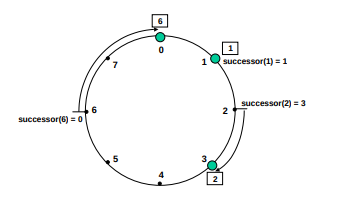
\includegraphics[width=10cm]{succ-pred.jpg}
	\caption{Aflarea succesorilor unor noduri}
\end{figure}

Un nod din reţea va fi responsabil de toate cheile aflate între nodul respectiv şi predecesorul său. De exemplu, pentru configuraţia din \textbf{Figure 1}, nodul 0 este responsabil de cheile ${4, 5, 6, 7}$, motivul fiind următorul: aflarea succesorului unui nod va avea, cu o mare probabilitate, complexitatea O(logN), deci în momentul în care aplicăm funcţia hash SHA-1 şi obţinem o cheie, pentru a găsi nodul responsabil de acea cheie vom apela funcţia $succesor(K)$ (unde $K$ este numărul format din primii 20 de biți ai hash-ului obținut), şi vom şti nodul la care vom pune valoarea asociată cheii.

Găsirea oricărui nod din reţea poate fi realizată dacă pentru fiecare nod se cunoaşte succesorul său, operaţia având complexitate $O(N)$, unde $N$ este numărul de servere. Pentru a eficientiza căutarea succesorului unui nod, în protocolul \textbf{Chord} se utilizează conceptul de "finger table": pentru fiecare nod se vor reţine $m$ câmpuri, al $i$-lea dintre acestea conţinând informaţia necesară pentru a găsi în reţea $succesor((n+2^{i-1})$ $mod 2^m)$. Cu ajutorul acestei tabele, succesorul unui nod va putea fi găsit în $O(logN)$.

\subsubsection{Integrarea protocolului în aplicaţie}

Utilizatorii ce doresc să partajeze un fişier vor insera în tabela hash distribuită un element ce are ca şi cheie primii M biţi din rezultatul funcţiei hash SHA-1 aplicate numelui fişierului, iar ca şi valoare informaţii despre nod. În acest mod, în momentul în care un client caută un fişier în reţea, dacă acesta este găsit, el va avea acces la detaliile despre nodul care partajează acel fişier şi îi va putea trimite un mesaj în care solicită descărcarea lui. Pentru a funcţiona corect, e suficient ca valoarea din DTH să fie numai portul şi adresa nodului, dar pot fi adăugate şi alte informaţii, pentru eficientizare. (de exemplu, poate fi reţinut şi tipul fişierului, pentru cazurile în care utilizatorul caută numai fişiere de un anumit tip, iar dacă acesta nu se potriveşte nu mai e nevoie să trimită alt mesaj)

Pentru a evita existența unor fișiere care apar în rețea ca fiind disponibile pentru a fi descărcate, însă serverele respective au ieșit din rețea, vor fi implentate două măsuri de siguranță: când serverul este închis voit, vor fi notificate nodurile din rețea care sunt responsabile de fișierele sale, pentru a le elimina din DTH, iar fiecare nod va rula din când în când o funcție prin care verifică faptul că serverele ce partajează fișierele de care este responsabil rulează.

\section{Detalii de implementare}

Vor fi implementate două aplicaţii: una de tip client (care va permite numai descărcarea fişierelor), şi una de tip server (va putea fi utilizată atât pentru descărcarea fişierelor, cât şi pentru distribuirea lor). Ambele aplicaţii vor face parte din reţeaua \textbf{Chord}, mai exact, ambele vor avea 2 thread-uri principale: unul dintre acestea va prelua comenzi de la tastatură (deci va fi cel cu care va interacţiona utilizatorul), iar cel de-al doilea va asigura funcţionalitatea reţelei Chord, iar în cazul aplicaţiei server va trimite, în plus, fişiere clienţilor interesaţi.

Codul din main a ambelor aplicații va avea, în mare, următoarea structură:

\begin{figure}[!h]
	\centering
	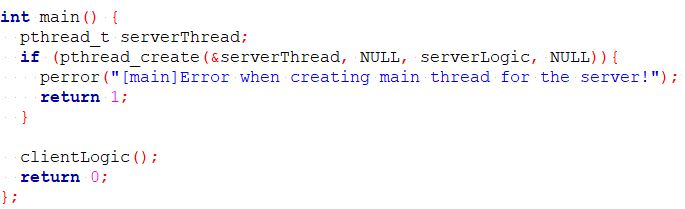
\includegraphics[width=10cm]{main.jpg}
	\caption{Structură main}
\end{figure}

Partea client (care citește comenzile și execută comenzi) a fiecărei aplicații:

\begin{figure}[!h]
	\centering
	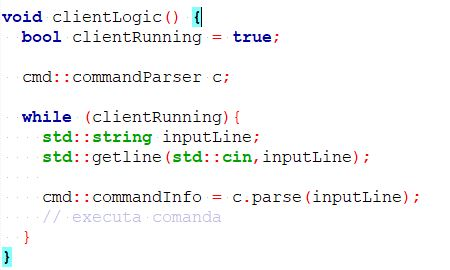
\includegraphics[width=6cm]{client.jpg}
\end{figure}

Partea server a fiecărei aplicații (funcția treat va primi ca unic parametru descriptorul socket corespunzător clientului):

\begin{figure}[!h]
	\centering
	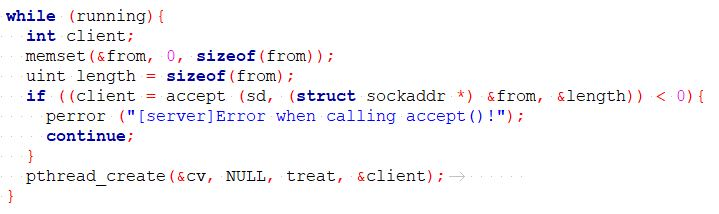
\includegraphics[width=10cm]{server.jpg}
\end{figure}

\begin{figure}[!h]
	\centering
	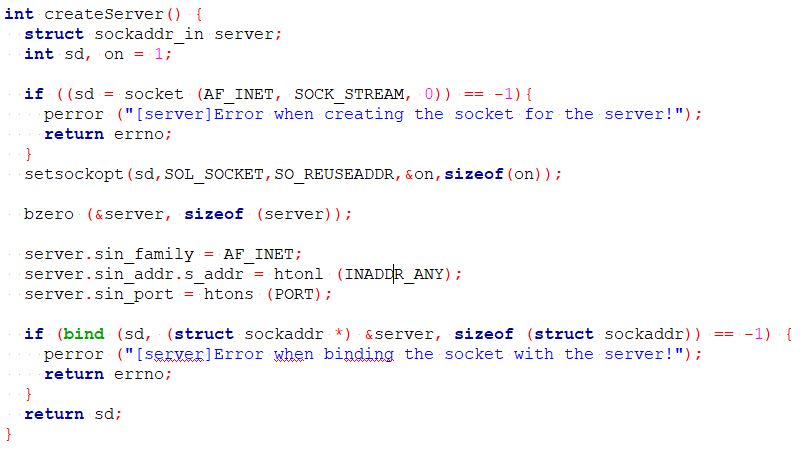
\includegraphics[width=10cm]{server-creation.jpg}
	\caption{Crearea serverului TCP}
\end{figure}

\begin{figure}[!h]
	\centering
	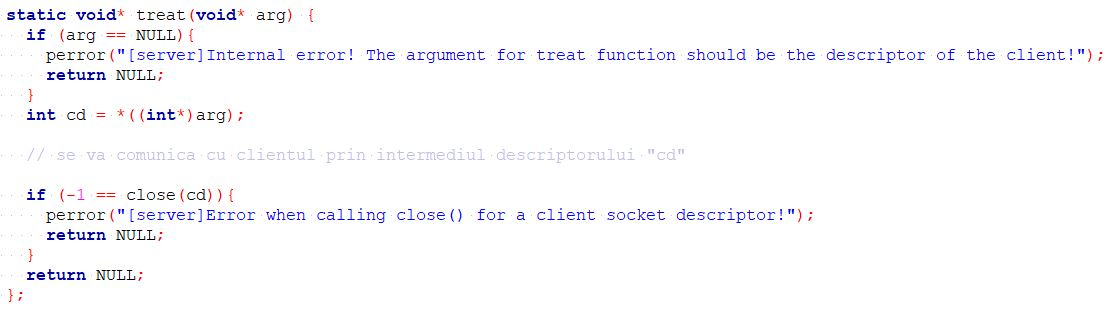
\includegraphics[width=14cm]{server-client-logic.jpg}
	\caption{Schema generală de rezolvare a cererilor clienților}
\end{figure}

\subsection{Modulele din proiect}

Pe partea de server (unul dintre cele 2 thread-uri principale ale fiecărei dintre aplicații) vor exista 2 module: unul va asigura funcționarea corectă a protocolului \textbf{Chord}, iar celălalt va permite partajarea fișierelor din sistemul de fișiere cu clienții ce trimit cereri pentru acest lucru. 

Pe partea de client (cel de-al doilea thread principal al unei aplicații) vor exista de asemenea 2 module: primul va permite căutarea și descărcarea fișierelor, iar cel de-al doilea va pune la dispoziție comenzi pentru partajarea în rețea a fișierelor. 

Aplicația de tip server va include toate cele 4 module (cu ajutorul ei utilizatorul va avea acces la toate funcționalitățile din aplicație), iar cea de tip client va avea integrat câte un modul din fiecare categorie de mai sus. (cel ce asigură funcționarea corectă a protocolului \textbf{Chord} și cel prin intermediul cărora vor putea fi descărcate fișiere din rețea)

Utilizatorii vor interacționa cu aplicațiile prin intermediul unei console cu comenzi. Pentru asta, va fi implementat un modul ce va conține toată logica pentru procesarea comenzilor: va exista un mod în care vor putea fi adăugate cu ușurință informații pentru comenzi (opțiuni, restricții) și o clasă ce va prelua textul introdus și va întoarce un obiect ce va conține toate detaliile necesare pentru executarea comenzilor (ID-ul comenzii, opțiunile prezente și valorile lor).

\begin{figure}[!h]
	\centering
	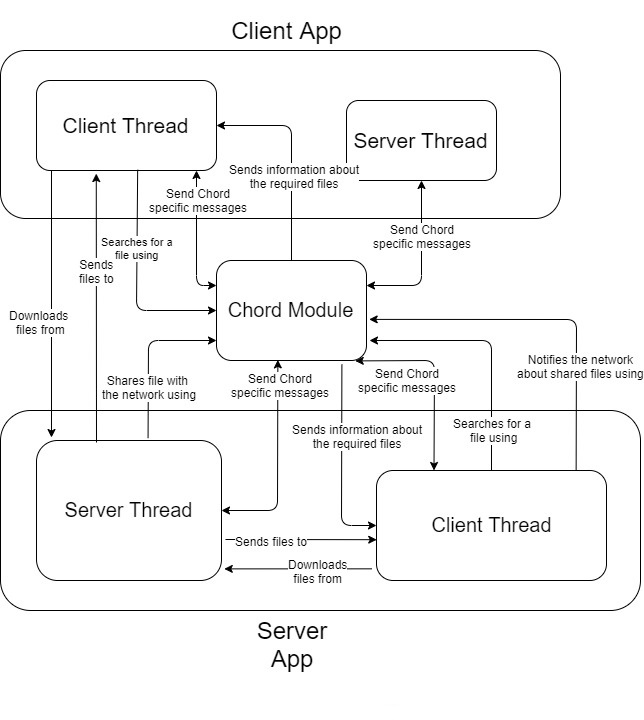
\includegraphics[width=12cm]{architecture.jpg}
	\caption{Arhitectura generală (ce include ambele aplicații)}
\end{figure}

\subsection{Chord}

Operațiile specifice protocolului \textbf{Chord} vor fi prezentate aici utilizând bucăți de pseudocod, preluat (la fel ca și imaginile) din lucrarea "Chord: A Scalable Peer-to-peer Lookup Service for Internet Applications" \cite{ChordArticle} (fiindcă prezentarea de cod \textbf{C++} ar presupune ca aplicația să fie deja implementată și funcțională).

\begin{figure}[!h]
	\centering
	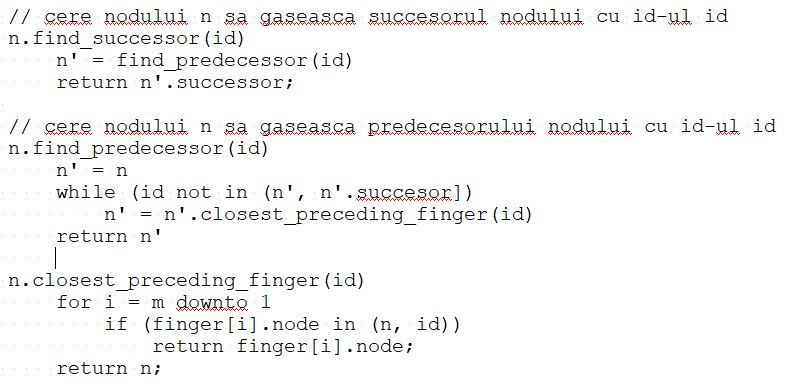
\includegraphics[width=14cm]{succesor.jpg}
	\caption{Pseudocod pentru găsirea succesorului unui id}
\end{figure}

\begin{figure}[!h]
	\centering
	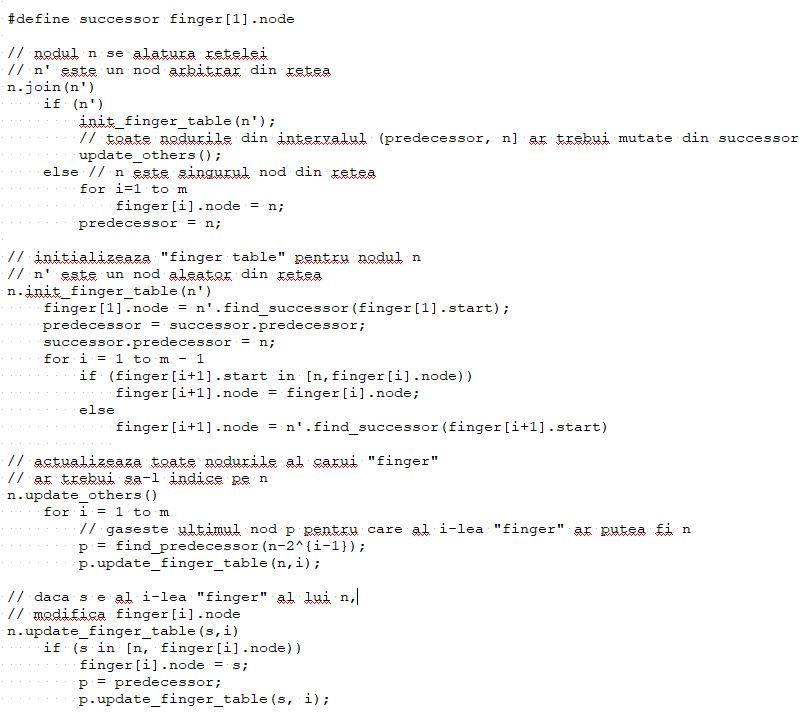
\includegraphics[width=14cm]{node-join.jpg}
	\caption{Pseudocod pentru intrarea unui nod în rețea}
\end{figure}

\begin{figure}[!h]
	\centering
	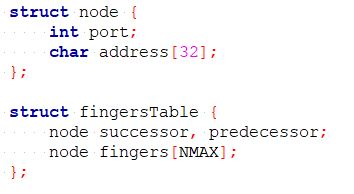
\includegraphics[width=7cm]{chord-structs.jpg}
	\caption{Declararea în C++ a tabelei "fingers table"}
\end{figure}

\newpage

\section{Scenarii de utilizare}

În aplicația client:

\begin{enumerate}
	\item Un utilizator poate căuta un fișier după nume, fiindu-i returnate toate fișierele găsite în rețea ce au numele respectiv
	\item Un utilizator poate filtra fișierele găsite după diferite criterii (tip, dimensiune)
	\item Un utilizator poate descărca oricare dintre fișierele găsite, moment în care va putea specifica și numele cu care să fie salvat fișierul la el în calculator
	\item Un utilizator poate vedea informații despre fișierele pe care le-a descărcat
	\item Un utilizator poate șterge direct din aplicație fișiere pe care le-a descărcat (dacă acestea încă se află în directorul în care au fost descărcate)
\end{enumerate}

În aplicația server toate cele de mai sus, iar în plus:

\begin{enumerate}
	\item Un utilizator poate adăuga un fișier din sistemul său de fișiere în rețea (pe care orice să-l poată descărca)
	\item Un utilizator poate crea o listă cu fișiere ce vor fi adăugate automat în rețea când acesta pornește aplicația (întrucât când aplicația e închisă, acestea nu sunt disponibile)
	\item Un utilizator poate edita acea listă cu fișiere
	\item Un utilizator poate elimina din rețea un fișier pe care l-a adăugat
	\item Un utilizator poate vedea de câte ori a fost descărcat unul dintre fișierele pe care acesta le-a adăugat
\end{enumerate}

\section{Îmbunătăţirea soluţiei propuse}

\subsection{Expresii regulate}

O îmbunătăţire a aplicaţiei ar fi posibilitatea de a căuta fişiere utilizând expresii regulate. Dacă informaţiile despre fişierele partajate din reţea ar fi ţinute toate pe un server central, atunci căutarea lor ar presupune în mare parte implementarea unui algoritm de potrivire al expresiilor regulate cu nişte şiruri de caractere. În reţeaua descentralizată descrisă în acest document lucrurile devin mai complicate: pentru a asigura faptul că operaţiile au complexitatea O(logN) cu o mare probabilitate, informaţiile despre serverul care partajează un fişier sunt ţinute într-un nod al reţelei, nod ales pe baza aplicării funcţiei hash SHA-1 pe numele fişierului. Mai exact, trebuie să ştim numele exact al fişierului pentru a putea găsi informații despre serverul de pe care putem să-l descărcăm. În continuare voi prezenta o variantă (şi o optimizare a acesteia) pentru căutarea unui fişier utilizând expresii regulate: 

\begin{enumerate}
	\item Căutăm fişierul respectiv pe fiecare server, aplicând un algoritm clasic de matching al expresiilor regulate, şi întoarcem toate rezultatele găsite. Complexitatea va fi O(n), întrucât vom parcurge toate nodurile din rețea folosindu-ne doar de câmpul "succesor".
	\item Pentru expresiile regulate în care singurul caracter special este $?$ (caracterul ce înlocuieşte exact un caracter, şi se potriveşte cu orice caracter din alfabetul peste care e construită expresia), în cazul în care numărul acestor caractere este mic (între 1 şi 4 de exemplu), se poate face o generate a tuturor combinaţiilor de şiruri de caractere ce se potrivesc cu pattern-ul, iar fiecare dintre acestea se caută cu complexitatea O(logN). Pentru toate celelalte pattern-uri se utilizează varianta de mai sus. Această optimizare poate fi implementată şi de sine stătătoare (deci permitem căutarea fişierelor al căror nume se potrivesc cu un pattern ce conţine cel mult 4 de $?$). Se va vedea o diferență de performanță dacă numărul nodurilor din rețea este mare.
\end{enumerate}

\subsection{Securitate}

\subsubsection{Criptare şi decriptare}

În tabela hash distribuită putem cripta informaţiile despre serverul ce partajează un fişier, utilizând un algoritm ce utilizează concepte precum cheie publică şi cheie privată (în acest mod adresa și portul serverului nu va putea fi văzute cu ochiul liber, ci doar după aplicarea algoritmului de decriptare, deci rețeaua este mai sigură).

\subsubsection{Parole / coduri secrete}

Putem limita accesul anumitor utilizatori la unele fişiere partajate prin posibilitatea de a adăuga o parola unui fişier, ce va trebui introdusă în momentul în care se face cererea de descărcare (în acest caz utilizatorii văd în continuare toate fişierele, dar e posibil să nu le poată descărca), sau putem ascunde complet unele fişiere, prin folosirea anumitor coduri în momentul căutării (cand introducem numele unui fişier căutat, pentru a-l găsi trebuie să introducem şi un anumit cod secret, pus de proprietar în momentul distribuirii fişierului în reţea).

\section{Concluzie}

Aplicația de partajare a fișierelor va furniza funcționalitățile de bază existente în orice aplicație de acest tip, iar folosirea protocolului \textbf{Chord} va asigura o complexitate bună a operațiilor ce vor fi executate la nivelul rețelei și scalabilitatea sistemului descentralizat, intrarea și ieșirea nodurilor din aceasta având impact mic asupra structurii (fapt demonstrat în lucrarea de prezentare a acestui protocol, "Chord: A Scalable Peer-to-peer Lookup Service for Internet Applications" \cite{ChordArticle}).

\begin{thebibliography}{9}
		
\bibitem{drawio}
\url{draw.io}
		
\bibitem{Chord}
\url{https://en.wikipedia.org/wiki/Chord_(peer-to-peer)}
		
\bibitem{ChordArticle}
\url{https://pdos.csail.mit.edu/papers/chord:sigcomm01/chord_sigcomm.pdf}		
\bibitem{PeerToPeer}
\url{https://profs.info.uaic.ro/~computernetworks/files/11rc_ParadigmaP2P_Ro.pdf}		
		
\end{thebibliography}

\end{document}